%-----------------------------------------------------------------------------------------------------------------------------------------------%
%	The MIT License (MIT)
%
%	Copyright (c) 2021 Jitin Nair
%
%	Permission is hereby granted, free of charge, to any person obtaining a copy
%	of this software and associated documentation files (the "Software"), to deal
%	in the Software without restriction, including without limitation the rights
%	to use, copy, modify, merge, publish, distribute, sublicense, and/or sell
%	copies of the Software, and to permit persons to whom the Software is
%	furnished to do so, subject to the following conditions:
%	
%	THE SOFTWARE IS PROVIDED "AS IS", WITHOUT WARRANTY OF ANY KIND, EXPRESS OR
%	IMPLIED, INCLUDING BUT NOT LIMITED TO THE WARRANTIES OF MERCHANTABILITY,
%	FITNESS FOR A PARTICULAR PURPOSE AND NONINFRINGEMENT. IN NO EVENT SHALL THE
%	AUTHORS OR COPYRIGHT HOLDERS BE LIABLE FOR ANY CLAIM, DAMAGES OR OTHER
%	LIABILITY, WHETHER IN AN ACTION OF CONTRACT, TORT OR OTHERWISE, ARISING FROM,
%	OUT OF OR IN CONNECTION WITH THE SOFTWARE OR THE USE OR OTHER DEALINGS IN
%	THE SOFTWARE.
%	
%
%-----------------------------------------------------------------------------------------------------------------------------------------------%

%----------------------------------------------------------------------------------------
%	DOCUMENT DEFINITION
%----------------------------------------------------------------------------------------

% article class because we want to fully customize the page and not use a cv template
\documentclass[a4paper,12pt]{article}

%----------------------------------------------------------------------------------------
%	FONT
%----------------------------------------------------------------------------------------

% % fontspec allows you to use TTF/OTF fonts directly
% \usepackage{fontspec}
% \defaultfontfeatures{Ligatures=TeX}

% % modified for ShareLaTeX use
% \setmainfont[
% SmallCapsFont = Fontin-SmallCaps.otf,
% BoldFont = Fontin-Bold.otf,
% ItalicFont = Fontin-Italic.otf
% ]
% {Fontin.otf}

%----------------------------------------------------------------------------------------
%	PACKAGES
%----------------------------------------------------------------------------------------
\usepackage{url}
\usepackage{parskip} 	

%other packages for formatting
\RequirePackage{color}
\RequirePackage{graphicx}
\usepackage[usenames,dvipsnames]{xcolor}
\usepackage[scale=0.9]{geometry}

%tabularx environment
\usepackage{tabularx}

%for lists within experience section
\usepackage{enumitem}

% centered version of 'X' col. type
\newcolumntype{C}{>{\centering\arraybackslash}X} 

%to prevent spillover of tabular into next pages
\usepackage{supertabular}
\usepackage{tabularx}
\newlength{\fullcollw}
\setlength{\fullcollw}{0.47\textwidth}

%custom \section
\usepackage{titlesec}				
\usepackage{multicol}
\usepackage{multirow}

%CV Sections inspired by: 
%http://stefano.italians.nl/archives/26
\definecolor{sectioncolor}{RGB}{0, 102, 204}  % Define blue color for sections
\titleformat{\section}{\Large\scshape\raggedright\color{sectioncolor}}{}{0em}{}[\titlerule]
\titlespacing{\section}{0pt}{10pt}{10pt}

%for publications
\usepackage[style=authoryear,sorting=ynt, maxbibnames=2]{biblatex}

%Setup hyperref package, and colours for links
\usepackage[unicode, draft=false]{hyperref}
\definecolor{linkcolour}{rgb}{0,0.2,0.6}
\hypersetup{colorlinks,breaklinks,urlcolor=linkcolour,linkcolor=linkcolour}
\addbibresource{citations.bib}
\setlength\bibitemsep{1em}

%for social icons
\usepackage{fontawesome5}

%debug page outer frames
%\usepackage{showframe}


% job listing environments
\newenvironment{jobshort}[2]
    {
    \begin{tabularx}{\linewidth}{@{}l X r@{}}
    \textbf{#1} & \hfill &  #2 \\[3.75pt]
    \end{tabularx}
    }
    {
    }

\newenvironment{joblong}[2]
    {
    \begin{tabularx}{\linewidth}{@{}l X r@{}}
    \textbf{#1} & \hfill &  #2 \\[3.75pt]
    \end{tabularx}
    \begin{minipage}[t]{\linewidth}
    \begin{itemize}[nosep,after=\strut, leftmargin=1em, itemsep=3pt,label=--]
    }
    {
    \end{itemize}
    \end{minipage}    
    }



%----------------------------------------------------------------------------------------
%	BEGIN DOCUMENT
%----------------------------------------------------------------------------------------
\begin{document}

% non-numbered pages
\pagestyle{empty} 

%----------------------------------------------------------------------------------------
%	TITLE
%----------------------------------------------------------------------------------------

% \begin{tabularx}{\linewidth}{ @{}X X@{} }
% \huge{Your Name}\vspace{2pt} & \hfill \emoji{incoming-envelope} email@email.com \\
% \raisebox{-0.05\height}\faGithub\ username \ | \
% \raisebox{-0.00\height}\faLinkedin\ username \ | \ \raisebox{-0.05\height}\faGlobe \ mysite.com  & \hfill \emoji{calling} number
% \end{tabularx}

\begin{tabularx}{\linewidth}{@{} X r @{}}
\Huge{Pengyuan Wang} & \multirow{8}{*}{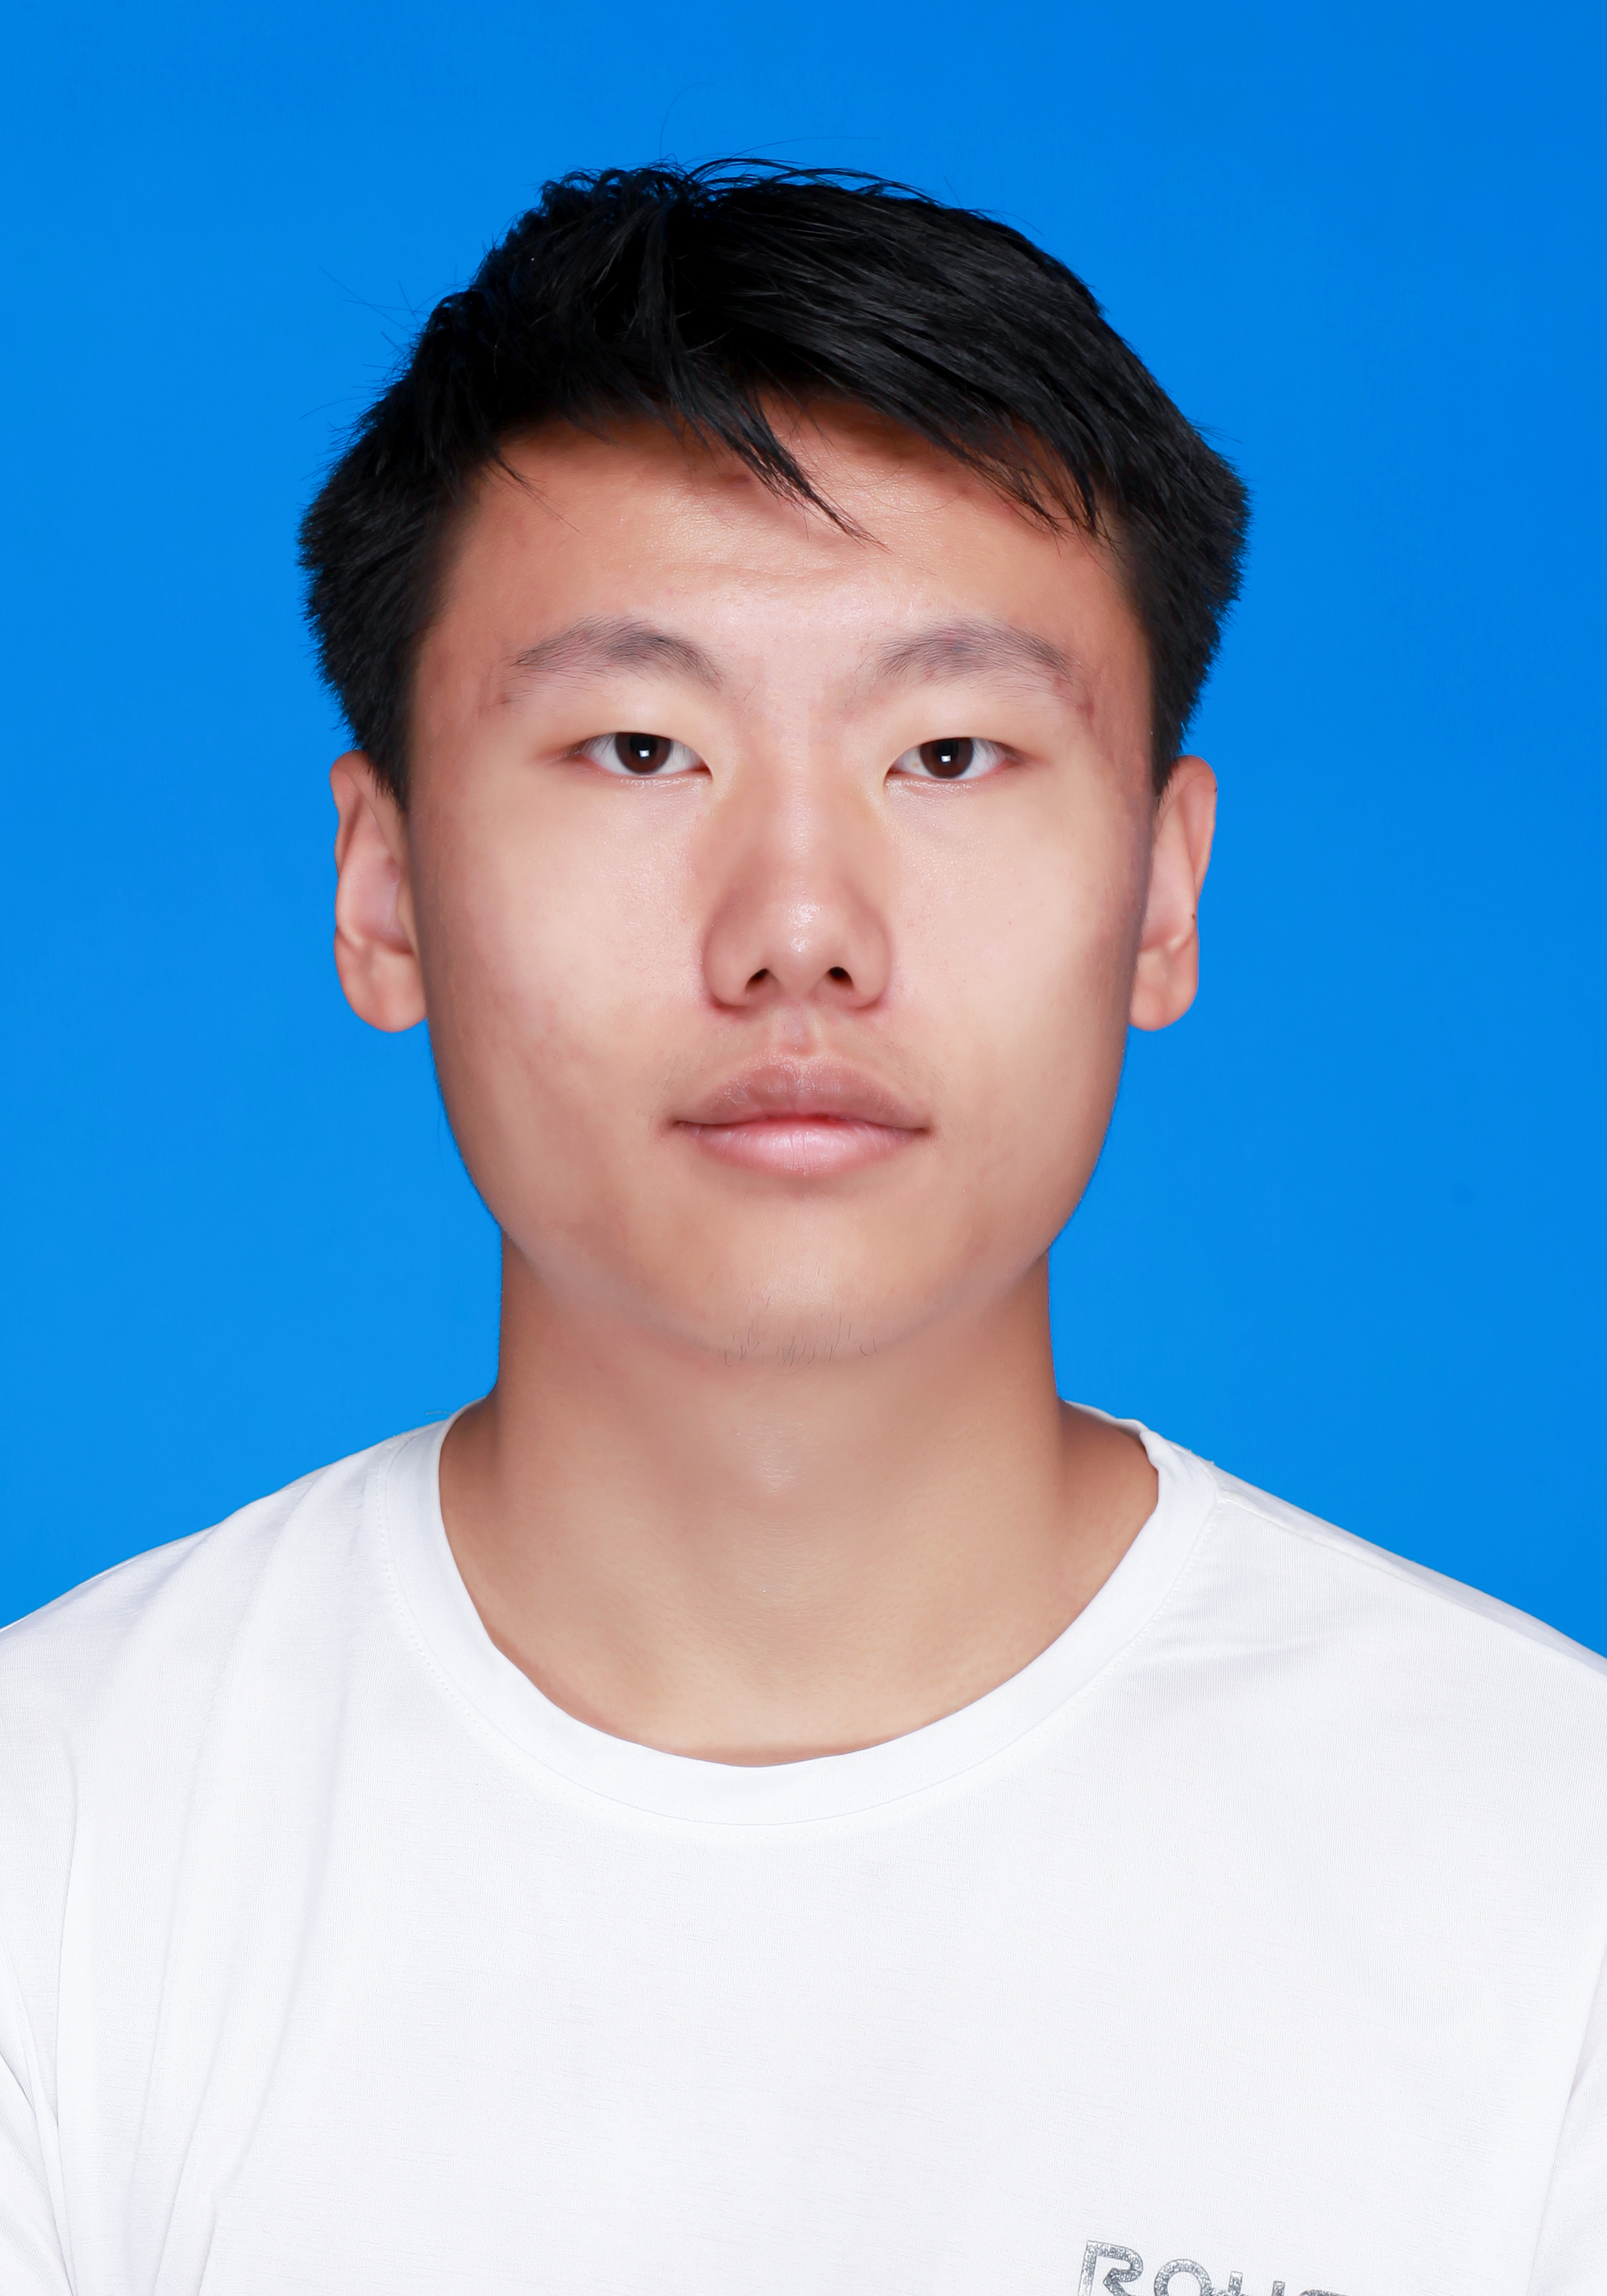
\includegraphics[width=3cm]{profile.jpg}} \\[3pt]
\normalsize{\textit{Undergraduate}} & \\
\normalsize{\textit{Zhejiang University, Robotics Engineering}} & \\[10pt]
\href{mailto:wpy.wangpengyuan@gmail.com}{\raisebox{-0.05\height}\faEnvelope \ wpy.wangpengyuan@gmail.com} \ $|$ \ 
\href{tel:+8618858112270}{\raisebox{-0.05\height}\faMobile \ (+86) 18858112270} & \\[3pt]
\href{https://nightcat204.github.io}{\raisebox{-0.05\height}\faGlobe \ nightcat204.github.io} \ $|$ \ 
\href{https://github.com/NightCat204}{\raisebox{-0.05\height}\faGithub\ NightCat204} & \\
\end{tabularx}
\vspace{10pt}

%----------------------------------------------------------------------------------------
% EXPERIENCE SECTIONS
%----------------------------------------------------------------------------------------

\section{Summary}
I am currently a third-year undergraduate student at Zhejiang University, majoring in Robotics Engineering and guided by Prof. Qiuguo Zhu. My research interests lie primarily in Legged Robot and Reinforcement Learning. I am also passionate about exploring more research areas.

%----------------------------------------------------------------------------------------
%	EDUCATION
%----------------------------------------------------------------------------------------
\section{Education}
\begin{tabularx}{\linewidth}{@{}l X@{}}	
2023 - 2027 & Bachelor of Engineering in Robotics Engineering at \textbf{Zhejiang University} \hfill \normalsize \\
& College of Control Science and Engineering \\
& Advisor: Prof. Qiuguo Zhu \\
\end{tabularx}

%----------------------------------------------------------------------------------------
%	HONORS AND AWARDS
%----------------------------------------------------------------------------------------
\section{Honors \& Awards}
\begin{tabularx}{\linewidth}{@{}l X@{}}
2024, 2025 & \textbf{First Prize}, National University Robot Competition "RoboMaster Super Match - National Championship" \\
& 2024 (National Top 4), 2025 (National Top 8) \\[3.75pt]
2024 & \textbf{First Prize}, Zhejiang University Robot Competition (Runner-up) \\[3.75pt]
2024, 2025 & \textbf{Third-Class Scholarship} (Top 20\% Students), Zhejiang University \\
\end{tabularx}

%Experience
\section{Research Experience}

\begin{joblong}{Humanoid Robot Control with Reinforcement Learning}{Mar 2025 - Present}
\item Developing running controllers for a humanoid robot using reinforcement learning
\item Configured simulation environments and trained open-source models
\item Designed reward functions to achieve stable locomotion
\item Gained foundational understanding of neural networks and reinforcement learning
\item Improved practical skills in simulation, algorithm design, and implementation using PyTorch and IsaacGym
\end{joblong}

\begin{joblong}{High-Maneuverability Drone Control System}{Jul 2025 - Sep 2025}
\item Contributed to developing a drone control system integrating Jetson ORIN NX and nxtpx4 flight controller
\item Implemented cascade PID architecture for decoupled position, velocity, and angular rate control
\item Applied PPO-based reinforcement learning with domain randomization for sim-to-real transfer
\item Achieved complex maneuvers including figure-eight trajectories
\item Strengthened practical skills in embedded systems programming and ROS-based integration
\end{joblong}

\begin{joblong}{Autonomous Navigation System Development}{Jul 2024 - Aug 2024}
\item Developed an autonomous navigation system for a wheeled robot using ROS under guidance of Prof. Yu Zhang
\item Implemented LiDAR-based SLAM for mapping
\item Integrated TEB and Far Planner for trajectory optimization
\item Enabled autonomous navigation and mapping in laboratory setting
\item Gained hands-on skills in the ROS ecosystem and practical understanding of SLAM and path planning
\end{joblong}
  
%Projects
\section{Projects}

\begin{tabularx}{\linewidth}{ @{}l r@{} }
\textbf{RoboMaster Competition: Infantry \& Aerial Robot Control Systems} & \hfill \href{https://nightcat204.github.io/project/}{Oct 2023 - Aug 2025} \\[3.75pt]
\multicolumn{2}{@{}X@{}}{Led the electrical control development for Infantry and Aerial robots over two seasons. Responsibilities spanned from low-level hardware development (circuit design and soldering) to advanced software implementation. Applied and optimized classical control methods such as PID, LQR, and MPC to meet specific task requirements, achieving high-performance motion control. This experience solidified programming foundation and deepened interest in robot control through hands-on system integration and teamwork.}  \\
\end{tabularx}

\begin{tabularx}{\linewidth}{ @{}l r@{} }
\textbf{Vision-Based Waste Sorting Robot} & \hfill \href{https://nightcat204.github.io/project/}{Aug 2024 - Sep 2024} \\[3.75pt]
\multicolumn{2}{@{}X@{}}{Contributed to developing a mecanum-wheeled sorting robot integrating LiDAR SLAM, stereo depth camera, and OpenCV-based color recognition for autonomous waste classification and transportation. Implemented URDF modeling for Gazebo simulation and established ROS communication architecture for module integration. Strengthened practical skills in Linux-based robotics tools including RViz, Gazebo, and Docker.}  \\
\end{tabularx}

\begin{tabularx}{\linewidth}{ @{}l r@{} }
\textbf{Zhongkong Cup: Autonomous Line-Following Robot} & \hfill \href{https://nightcat204.github.io/project/}{Mar 2024 - May 2024} \\[3.75pt]
\multicolumn{2}{@{}X@{}}{As team leader, led the development of an autonomous line-following robot. Primarily responsible for mechanical design and control algorithm deployment. The robot utilized grayscale sensors for navigation and featured custom-designed mechanisms, including a bucket and robotic arm, to perform object manipulation tasks. Gained practical experience in mechanical modeling and control algorithm implementation.}  \\
\end{tabularx}

%----------------------------------------------------------------------------------------
%	PUBLICATIONS
%----------------------------------------------------------------------------------------
% \section{Publications}
% \begin{refsection}[citations.bib]
% \nocite{*}
% \printbibliography[heading=none]
% \end{refsection}

%----------------------------------------------------------------------------------------
%	SKILLS
%----------------------------------------------------------------------------------------
\section{Skills}
\begin{tabularx}{\linewidth}{@{}l X@{}}
Programming Languages & \normalsize{C/C++, Python, MATLAB}\\
Robotics Tools & \normalsize{ROS, Gazebo, RViz, IsaacGym}\\
Control Theory & \normalsize{PID, LQR, MPC}\\
Machine Learning & \normalsize{Reinforcement Learning (PPO), PyTorch}\\
Embedded Systems & \normalsize{STM32, Jetson ORIN NX, Embedded Linux}\\
\end{tabularx}

\vfill
\center{\footnotesize Last updated: \today}

\end{document}
